\documentclass[../main.tex]{subfiles}
\graphicspath{{\subfix{../diagrams/}}}
\usepackage{float}

\begin{document}
\subsection{Aims \& Purpose}
The purpose of the system is to provide a web and mobile application for grocery shopping and delivery. It allows the client to browse available products and place orders on them. They can also create sets of favorite products in order to facilitate future browsing. When the order is placed, the client can view the status of the order and communicate with the courier. The system also includes an interface for shop employees to prepare and dispatch orders.

\subsection{Modules}
The system comprises three modules:
\begin{enumerate}
    \item Client % -- this module includes client-facing features, such as browsing products and placing orders
    \item Delivery % -- serves as a bridge between the shop and the client; contains functionality regarding the delivery of placed orders
    \item Shop % -- this module is responsible for managing the inventory and processing orders
\end{enumerate}

Each module takes part in the process of fulfilling an order. To describe each module's functionality, let us analyze the use cases of the system.

\subsection{Architecture}



As shown in the next diagram, system has typical microservice structure with backend, web app and mobile app. Backend consist of three independent modules (each with its own database). Modules communicate with each other using REST protocol.

Furthermore, communication between backend and frontend runs through Api gateway, which is single entry point for all client applications. Api gateway connects also with Identity provider (e.g. Identity Server, Google), that is the source of JWT tokens needed to authenticate to the backend. Information about specific users is stored in Users database in the backend.

There are two client applications: mobile and web. Mobile app is the one, that will be used by the most users to place orders. It will be also used by the couriers to manage delivery process and by the shop employees to prepare orders. 

Web app has customer view with the same functionalities as the mobile app. It also contains shop manager view, which is used by managers to change products offer and add new shop units to the system.

\newpage

\begin{figure}[h!]
\caption{High level system structure.}
\vspace{5mm}
\centering
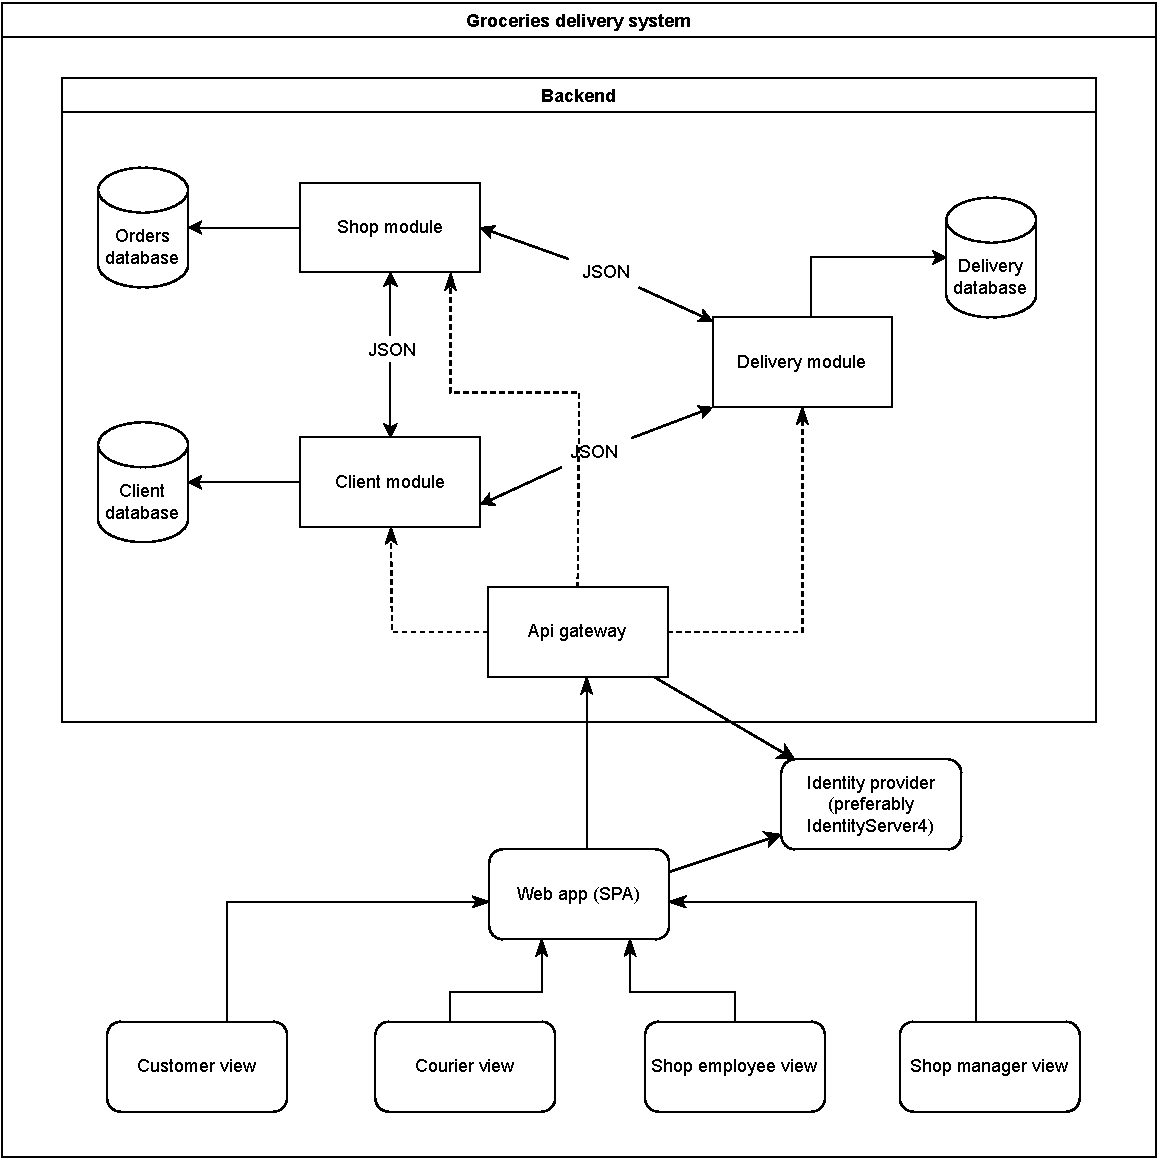
\includegraphics[width=\textwidth]
{diagrams/architecture.pdf}
\end{figure}

\subsection{Technological stack}

The backend consists of three independent modules, that implement business logic, one api gateway and four databases. Each module and api gateway should be implemented in a technology, that allows creating REST apis (e.g ASP.NET, Node). Databases should be relational (e.g. SQL Server, PostreSQL).

Web client app should be a Single Page Application (e.g. React, Angular), which implements OAuth 2.0 flow. Lastly, mobile app should be written in a technology, that is cross-platform (like React Native, Flutter).

The whole system, including databases and client apps should be deployed to the cloud (e.g. Azure) and ideally use some kind of containerization (Docker).

\subsection{Authorization}

Application should use OAuth 2.0 end user authentication (preferably IdentityServer4 with username and password). The auth flow should be Authorization Code Flow with PKCE, because our web app is a Single-Page-Application (most likely written in React or Angular) and secrets can't be used in the source code.

\subsection{User Stories}

In total, there are five actors in the system: the client, the courier, the shop employee, the shop manager (which is also a shop employee) and the algorithm. The system provides each actor with functionalities included in Table~\ref{tab:user_stories}. Note that the algorithm doesn't have an explicit user interface and, as such, shall be effectively transparent to other users. 

\begin{table}[h!]
    \centering
    \begin{tabular}{l|l|l|l}
        \toprule
        \textbf{As a...} & \textbf{I want to...} & \textbf{So that...} & \textbf{MoSCoW} \\
        \midrule
        Client & create an account & I can place orders & must \\
        & browse products & I know what to buy & must \\
        & make an order & I can inform the shop what I want & must \\
        & add favorite sets & I can speed up future shopping & could \\
        & choose time of delivery & I can easily collect it & should \\
        \midrule
        Courier & register an account & I can work & must \\
        & declare my availability & I can work when I can & must \\
        & accept orders & I can collect and deliver them & must \\
        & send messages to the client & I can communicate with them & should \\
        & deliver the order & I can fulfill the client's request & must \\
        & query the shop for new orders & I can choose an order to deliver & could \\
        & confirm goods received & I can mark the job as finished & must \\
        \midrule
        Shop employee & see products ordered by a client & I can complete orders & must \\
        & know how to mark orders & I can pack orders & should \\
        & change order's status & I can prepare orders and call couriers & must \\
        \midrule
        Shop manager & manage the list of products & I can update available products & must \\
        & check couriers' availability & I can make a schedule & must \\
        & see history of orders & I can generate reports & could\\
        \midrule
        Algorithm & I can assign couriers to orders & I can minimize delivery time & could \\
        & I can assign shops to orders &  & could \\
        & analyze couriers' position & & could \\
        \bottomrule
    \end{tabular}
    \caption{User stories}
    \label{tab:user_stories}
\end{table}

\newpage
\subsection{Use Cases}

\subsubsection{Client}
The main client functionality is placing orders. It includes:
\begin{itemize}
    \item viewing products
    \item adding and removing products from cart
    \item applying coupons to get discount
    \item choosing the payment method
    \item sending messages to courier
    \item making complaints when their requirements are not fulfilled
\end{itemize}
Client can also create the account and login so they can list their previous orders, track the current ones and save their contact detail and address data. They can also register loyalty card.

\subsubsection{Courier}
Courier can register an account and login. When logged he can deliver packages, that consists of:
\begin{enumerate}
    \item querying shop for pending orders
    \item accepting orders
    \item picking packages from the shop
    \item sending messages to client to inform them about package status updates (such as delays)
    \item notifying client when package is ready to collect
    \item confirming package received
\end{enumerate}
Courier also declare availability to inform shop when he can work.

\subsubsection{Shop employee}
The main role of shop employee is preparing orders. It consists of:
\begin{enumerate}
    \item accepting or rejecting the order placed by client
    \item packing products and addressing package
    \item marking when the order is ready to pick
    \item notifying courier
\end{enumerate}
Employee can also reports products shortage

\subsubsection{Shop manager}
Shop manager extends shop employee functionality. He also manages the list of offered products and chain of available stores. He can also view orders history and generate reports regarding shop efficiency.

\subsubsection{Algorithm}
Algorithm is responsible for assigning shop to order and courier to order. It should work in a way to minimize time difference between desired and predicted time of delivery and minimize courier waiting time.

\vspace{10mm}
\begin{figure}[h!]
\caption{Use case diagram.}
\vspace{5mm}
\centering
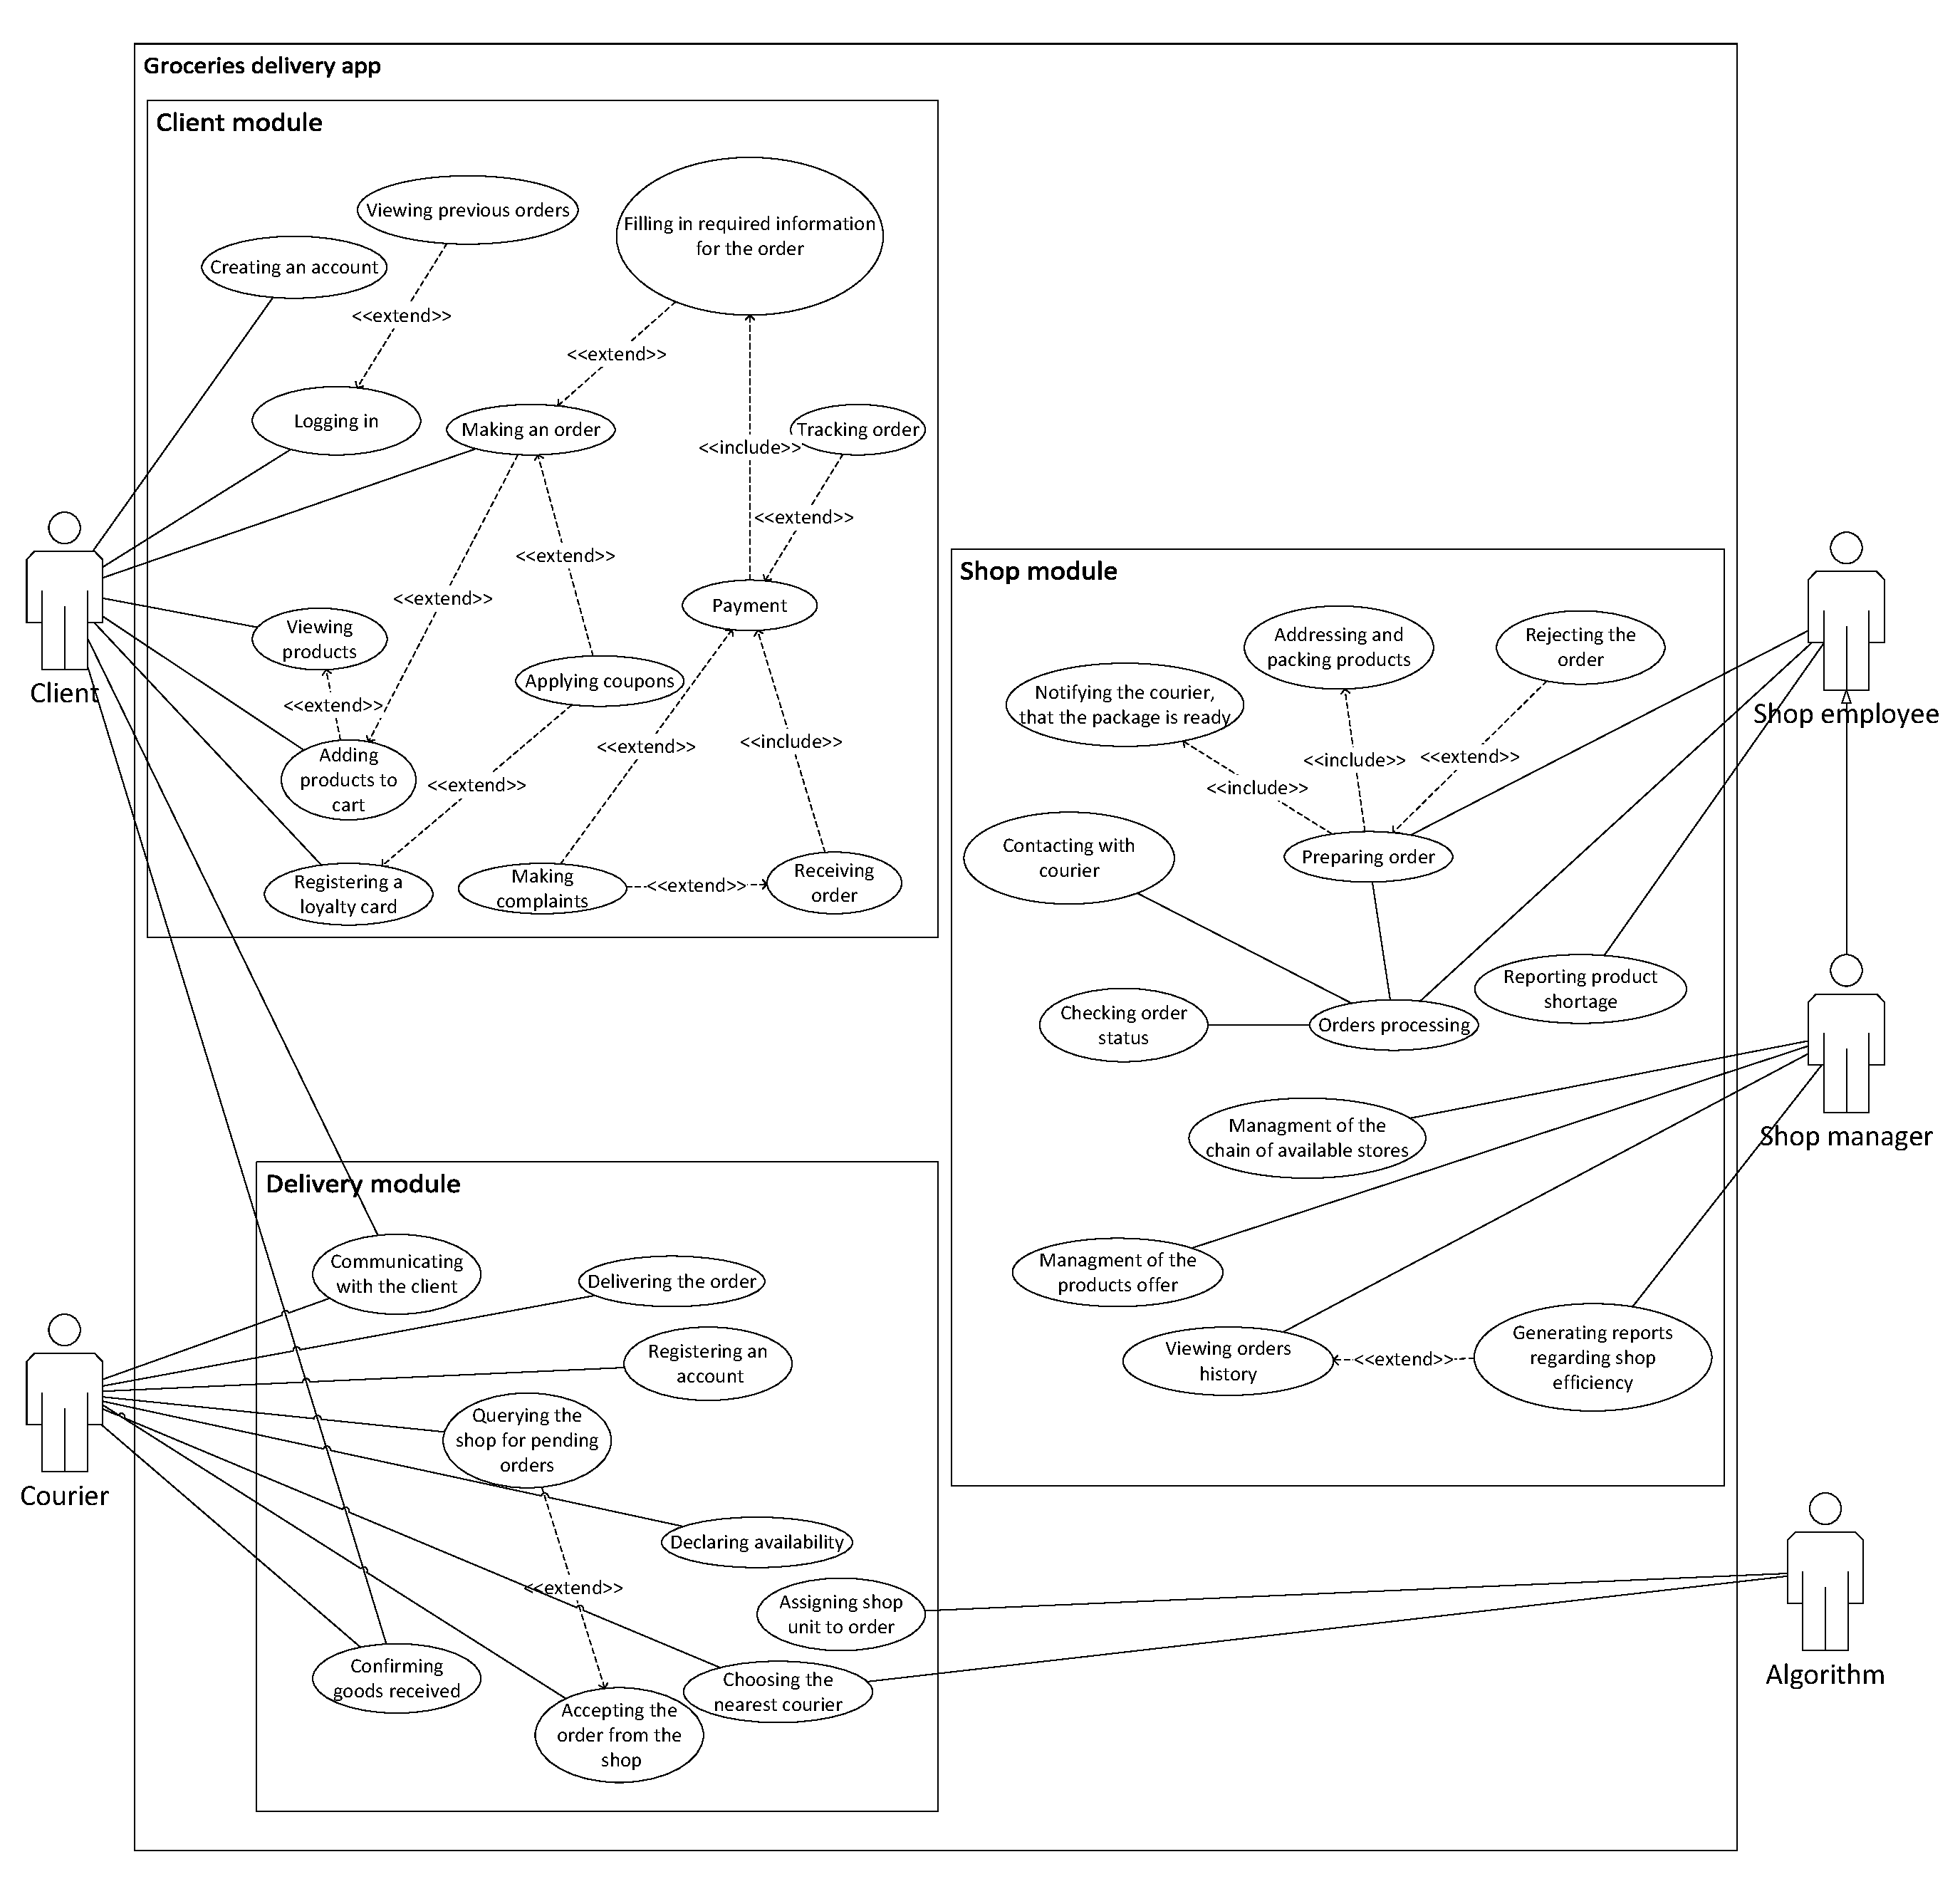
\includegraphics[width=1\textwidth]{use-case-diagram.pdf}
\end{figure}

% \makebox[\textwidth][c]{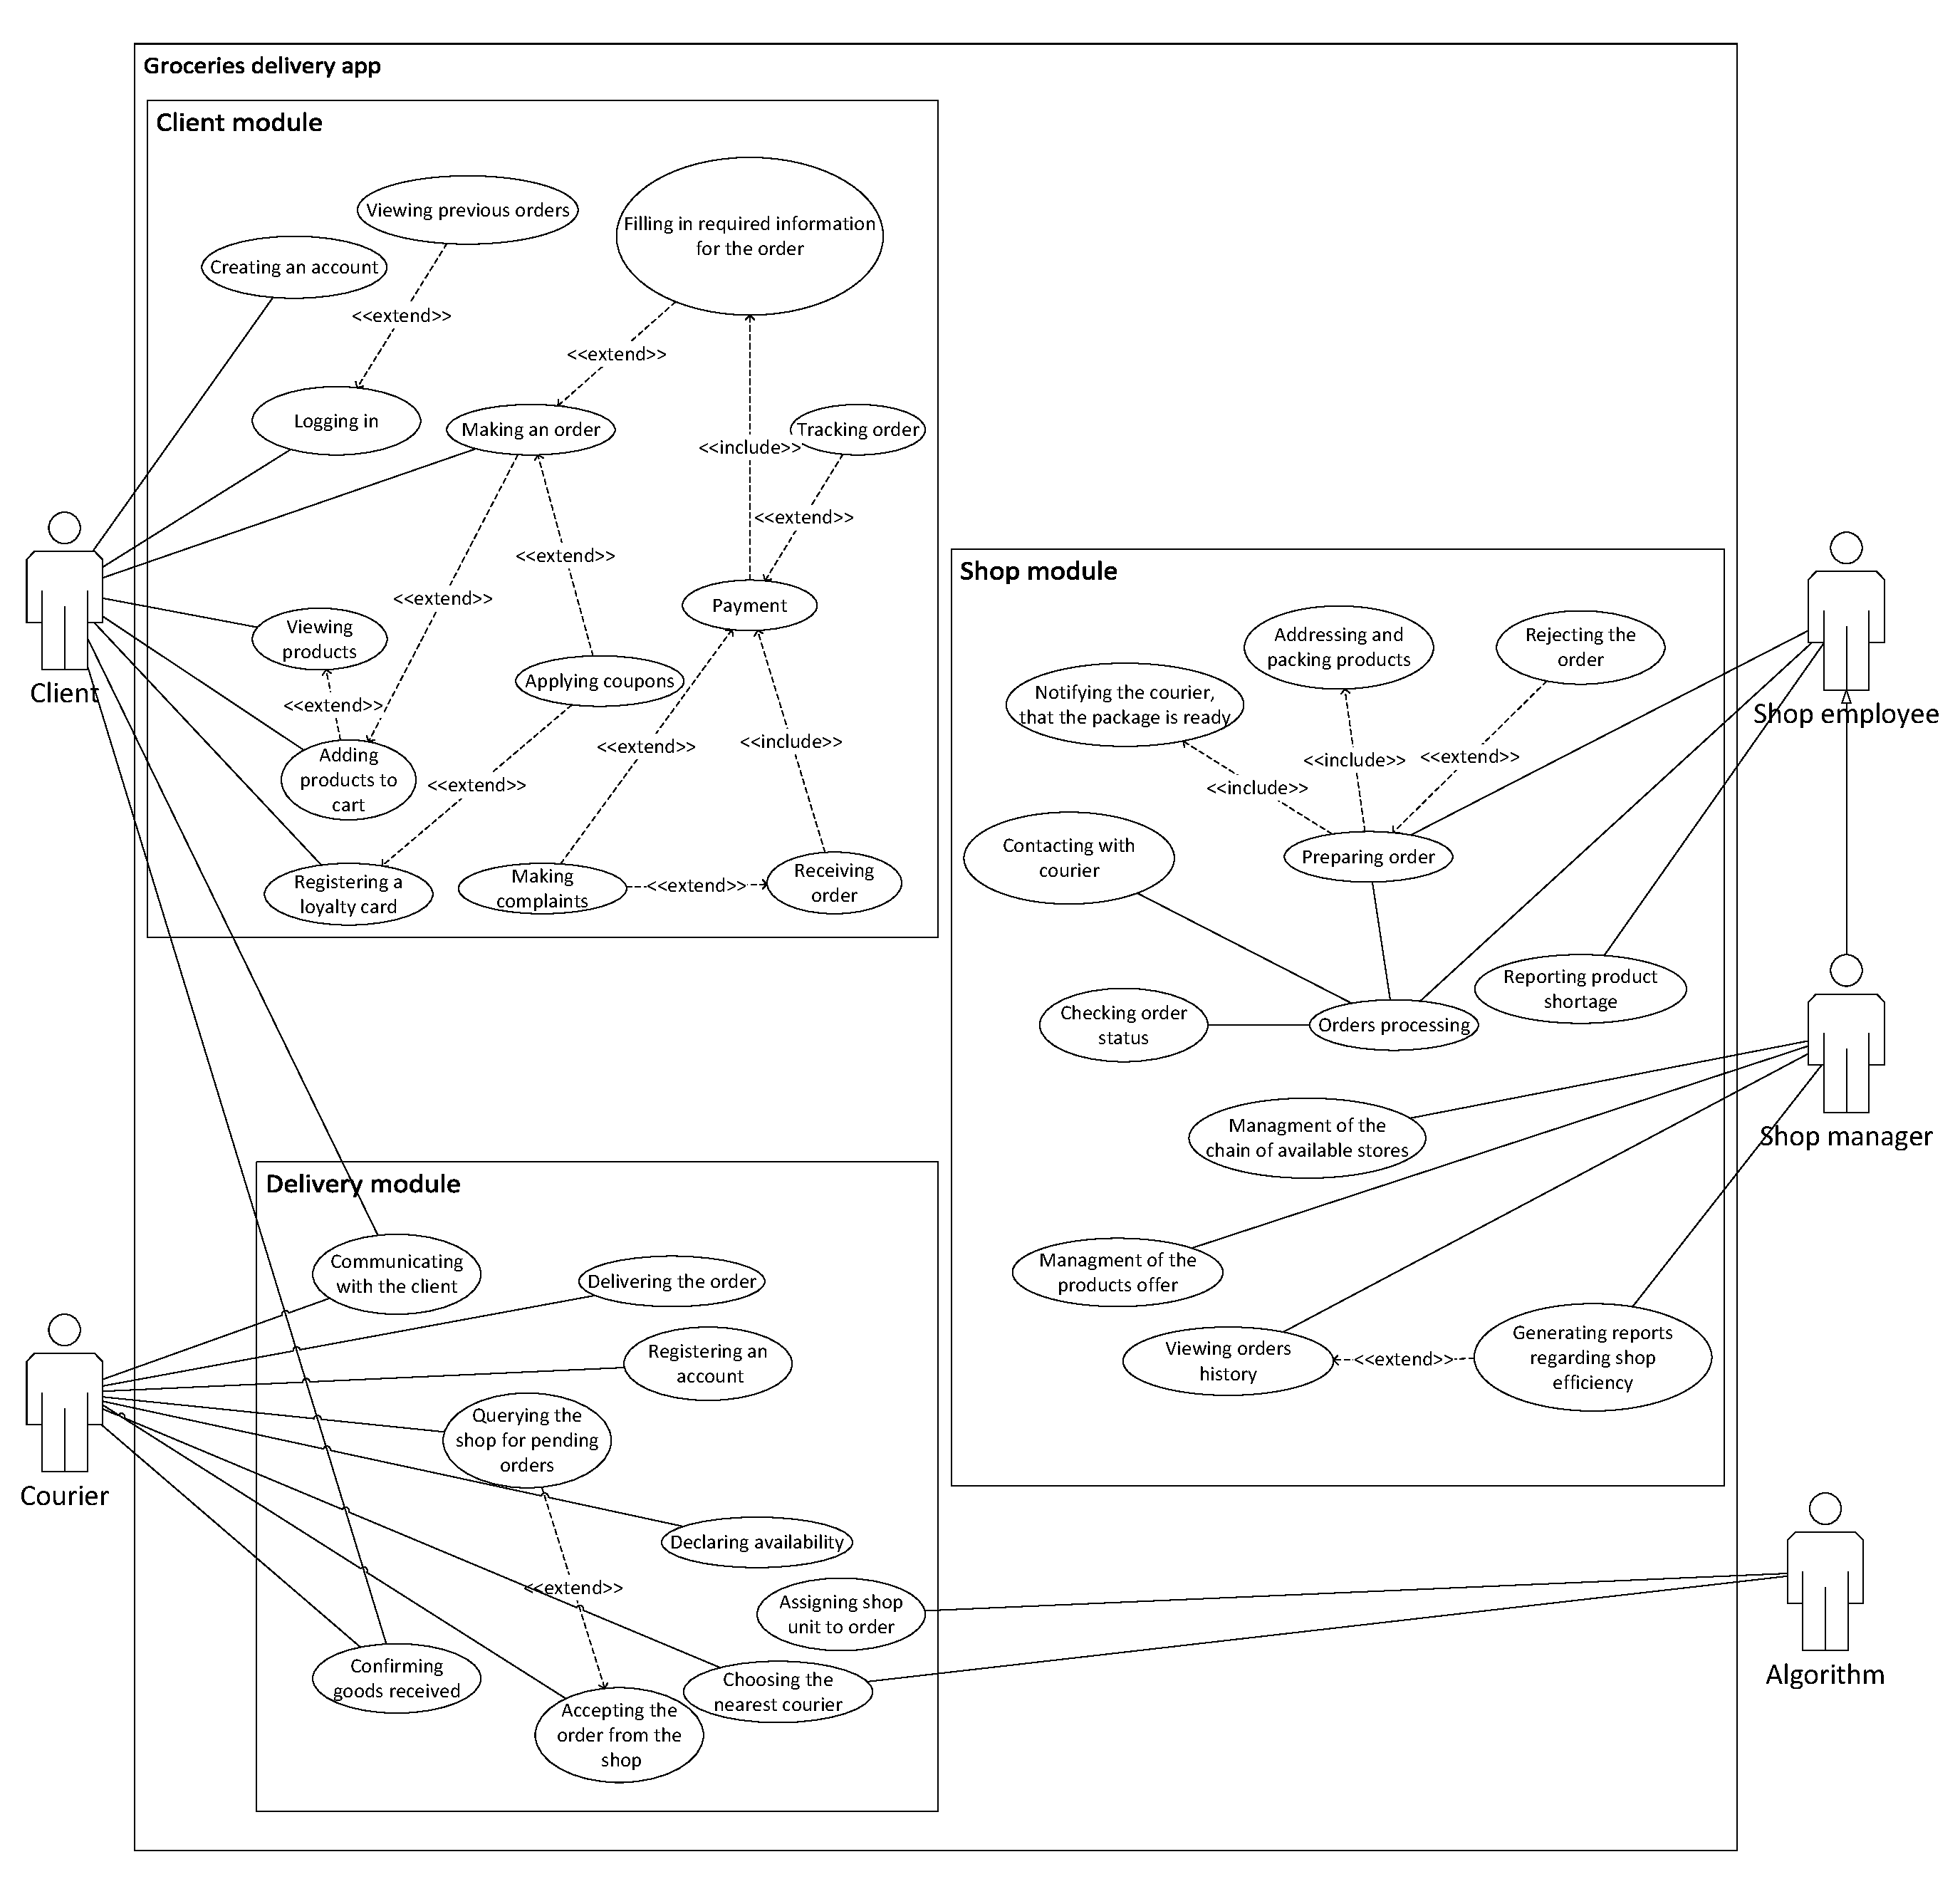
\includegraphics[width=1\textwidth]{use-case-diagram.pdf}}

\end{document}